\chapter{Considerações Gerais}
\label{cap:02}

\section{Engenharia de Software e Qualidade}

%Contextualiza o papel da Engenharia de Software no desenvolvimento moderno, discutindo importância da qualidade, confiabilidade, impacto dos defeitos e relação entre complexidade do software e dificuldade de verificação manual.
A Engenharia de Software compreende a aplicação de abordagens sistemáticas, disciplinadas e quantificáveis ao desenvolvimento, à operação e à manutenção de sistemas \citeonline{Valente2020}. Como a computação está presente em grande parte das atividades contemporâneas, assegurar a confiabilidade e a estabilidade das aplicações tornou-se uma exigência fundamental, e não apenas um diferencial técnico.

Embora os níveis de complexidade e os riscos envolvidos variem conforme o domínio, a aplicação de princípios de engenharia permanece indispensável. Essa necessidade é evidenciada em sistemas de segurança crítica, nos quais falhas de software podem resultar em consequências catastróficas. Um exemplo histórico notável é o caso do acelerador linear Therac-25, cujos erros de programação causaram acidentes fatais por superexposição à radiação \citeonline{turner1993investigation}.

A relevância da qualidade, porém, não se restringe a cenários de alto risco. Mesmo que um sistema de gestão de uma padaria não tenha a mesma complexidade ou criticidade de um sistema bancário, médico ou militar, ambos precisam ser confiáveis e sustentáveis ao longo do tempo. Em qualquer escala, o software deve preservar a experiência do usuário e a integridade dos processos que apoia.

A manutenção de padrões de qualidade em projetos colaborativos, portanto, torna-se um desafio crescente. À medida que um sistema evolui, a complexidade técnica e a densidade do código também aumentam, tornando processos de verificação exclusivamente manuais pouco viáveis e sujeitos a falhas humanas.

\section{Teste de Software}

%Apresenta conceitos fundamentais sobre testes, objetivos, limitações da inspeção manual e importância de detectar falhas antes da entrega. Explica a perspectiva de Myers e relaciona com a necessidade de suporte automatizado à verificação.
O teste de software busca, por meio de um conjunto finito de casos, verificar e validar (V\&V) se a aplicação atende aos requisitos esperados \cite{Valente2020}. Essa etapa representa um investimento significativo: cerca de 50\% do tempo e mais de 50\% do custo total do desenvolvimento de um sistema são consumidos pela atividade de testes \cite{Myers2014}.

Esse processo inicia-se em componentes individuais ou pequenos módulos, com o objetivo de identificar falhas lógicas e de dados. Após essa validação inicial, os componentes são integrados ao sistema para testes de ordem superior, cujo objetivo é assegurar que o software atenda aos requisitos do cliente \citeonline{Sommerville2019}. \citeonline{Myers2014} destaca que o teste não deve ser entendido como uma forma de demonstrar que o software funciona, mas como um processo de executá-lo com a intenção explícita de encontrar falhas. Nessa perspectiva, um ``teste bem-sucedido'' é aquele que revela um erro ainda não descoberto. Em sistemas cada vez mais complexos, aplicar essa abordagem apenas de forma manual torna-se exaustivo e sujeito a vieses, reforçando a necessidade de apoio automatizado.

\subsection{Teste Estrutural (Caixa Branca)}

%Descreve os princípios do teste estrutural, destacando sua análise da lógica interna do programa. Mostra por que ele é relevante para identificar caminhos independentes, estruturas condicionais e decisões do código.
O teste estrutural, também conhecido como teste de caixa branca, concentra-se na análise da lógica interna do programa \cite{Delamaro2013}. Ao contrário do teste de caixa preta, que observa se entradas e saídas correspondem ao esperado, essa técnica exige acesso ao código-fonte para avaliar caminhos de execução, \textit{loops} e condições lógicas.

Sua relevância reside na capacidade de orientar a verificação das estruturas internas do programa. Isso inclui apoiar a identificação de instruções, desvios lógicos (verdadeiro e falso), laços de repetição e caminhos independentes que devem ser considerados durante o planejamento dos testes.

\subsubsection{Grafo de Fluxo de Controle (GFC)}

%Explica o que é o GFC, seus elementos (nós, arestas, desvios), como representa a lógica interna de um programa e sua importância para análise estrutural. Introduz o uso do grafo em ferramentas de teste e análise estática.
O Grafo de Fluxo de Controle (GFC) é uma representação gráfica usada na análise estrutural. Ele modela a lógica do programa como um grafo dirigido, em que os \textbf{nós} representam blocos de processamento sequencial, sem desvios, e as \textbf{arestas} representam o fluxo de controle entre esses nós.

Entre os elementos do GFC estão os nós de predicado, que correspondem a pontos de decisão no código, como \texttt{if} ou \texttt{while}, dos quais partem múltiplas arestas. Ferramentas de teste e análise estática utilizam o GFC para calcular caminhos independentes e determinar a complexidade lógica do algoritmo, transformando o código textual em uma estrutura matemática navegável.

\pagebreak

Para consolidar o entendimento sobre a relação entre o código-fonte, o Grafo de Fluxo de Controle (GFC) e a Complexidade Ciclomática, apresenta-se a seguir um algoritmo simples de verificação condicional.

\lstinputlisting[language=Python, caption={Algoritmo de verificação condicional.}, label={lst:verifica_status}, numbers=left]{fontes/verificaStatus.py}

A partir da análise do Código \ref{lst:verifica_status}, é possível mapear a lógica para uma representação visual. A Figura \ref{fig:exemplo_gfc} ilustra o GFC correspondente, onde os blocos de comando tornam-se nós e o fluxo de execução torna-se arestas direcionadas.

\begin{figure}[H]
    \centering
      \caption{Exemplo de GFC.}
    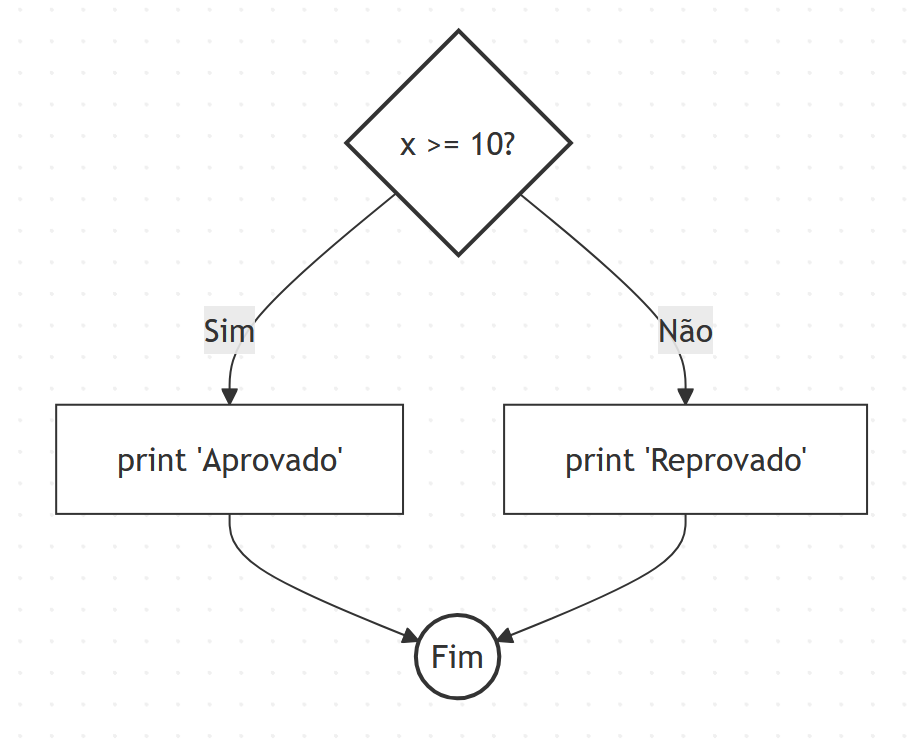
\includegraphics[width=0.5\linewidth]{imagens/diagramas/exemplo_gfc.png}

    \label{fig:exemplo_gfc}
    \fonte{Elaborada pelo autor.}
\end{figure}

\subsubsection{Complexidade Ciclomática - V(G)}

%Detalha a métrica proposta por McCabe, apresentando fórmula, interpretação, relação com quantidade de caminhos independentes e justificativa para sua adoção como indicador de complexidade lógica.
A Complexidade Ciclomática é uma métrica de software desenvolvida por Thomas McCabe em 1976. Ela quantifica a complexidade lógica de um programa a partir do número de caminhos linearmente independentes em seu Grafo de Fluxo de Controle \citeonline{McCabe1976}.

A métrica é calculada pela fórmula $V(G) = E - N + 2P$, em que $E$ é o número de arestas, $N$ é o número de nós e $P$ é o número de componentes conexos do grafo. Em grafos com apenas um componente conexo, essa expressão simplifica-se para $V(G) = E - N + 2$. O valor resultante $V(G)$ indica o número mínimo de casos de teste necessários para cobrir todos os caminhos independentes do código. McCabe sugere que módulos com complexidade superior a 10 são mais propensos a erros e difíceis de manter, justificando o uso dessa métrica como um indicador crítico de qualidade e testabilidade \citeonline{McCabe1976}.

\subsection{Cálculo da Complexidade Ciclomática}
Com base na representação visual da Figura \ref{fig:exemplo_gfc}, é possível aplicar a métrica de McCabe para determinar a complexidade lógica $V(G)$. Observando o grafo, identificam-se os seguintes elementos:

\begin{itemize}
    \item \textbf{Nós ($N$):} 4 (Início/If, Print Aprovado, Print Reprovado, Fim).
    \item \textbf{Arestas ($E$):} 4 (As conexões entre os nós).
    \item \textbf{Componentes conexos ($P$):} 1 (O grafo é único e interligado).
\end{itemize}

Aplicando a fórmula fundamental de McCabe:

\begin{equation}
    V(G) = E - N + 2P
\end{equation}

Substituindo pelos valores extraídos do grafo:

\[
    V(G) = 4 - 4 + 2(1) = 2
\]

O resultado $V(G) = 2$ indica que existem dois caminhos linearmente independentes no código: (1) o caminho em que a condição é verdadeira e (2) o caminho em que a condição é falsa. Esse valor confirma a baixa complexidade do algoritmo e indica que são necessários, no mínimo, dois casos de teste para cobrir a lógica da função.



\section{Análise Estática de Código}

%Introduz o conceito de análise sem execução (análise estática), justificando por que é adequada para inspeção estrutural. Diferencia análise estática de análise dinâmica e apresenta aplicações práticas.
A análise estática de código consiste no exame do software sem executá-lo. Essa técnica é adequada para a inspeção estrutural, pois permite verificar a base de código em busca de padrões sintáticos, violações de regras e métricas de complexidade ainda durante o desenvolvimento.

Diferencia-se da análise dinâmica, que requer a execução do programa com dados de teste reais para observar comportamentos em tempo de execução (como uso de memória e falhas). Aplicações práticas da análise estática incluem a detecção precoce de bugs, verificação de conformidade com guias de estilo (linting) e o cálculo automático de métricas como a complexidade ciclomática, permitindo feedback imediato ao desenvolvedor.

\subsection{Processamento Léxico e Sintático}

%Aborda conceitos de compiladores aplicados ao seu trabalho: tokenização, identificação de estruturas, análise sintática simplificada e como essas etapas são utilizadas na construção do GFC.
Para construir o GFC e realizar a análise estática, o GUY utiliza conceitos de compiladores. O processo inicia-se com a \textbf{tokenização} (análise léxica), que divide o código-fonte em unidades mínimas de significado (tokens) \citeonline{Cooper2012}.

Em seguida, realiza-se a identificação de estruturas através da \textbf{análise sintática}, que organiza esses \textit{tokens} em uma Árvore Sintática Abstrata (AST). A AST é uma representação hierárquica que expõe a estrutura gramatical do código \citeonline{Aho1995}. É percorrendo a AST que a ferramenta identifica onde começam e terminam os blocos lógicos (funções, loops, condicionais) para, a partir disso, desenhar os nós e arestas do GFC e calcular a complexidade.

\section{Tecnologias e Linguagens Adotadas}

%Apresenta as tecnologias que podem ser aplicadas no desenvolvimento da ferramenta web: frameworks front-end, back-end, bibliotecas de parsing, libs de visualização de grafos, e justificativas técnicas para as escolhas.
O GUY adota uma arquitetura de extensão para o \textit{Visual Studio Code} (VS Code). A lógica principal executa no \textit{Extension Host}, utilizando Node.js e TypeScript para acessar o arquivo aberto no editor, acionar a análise estática e coordenar a comunicação com a interface. Na camada visual, o framework \textbf{React.js} é utilizado em uma \textit{Webview}, permitindo a renderização interativa do Grafo de Fluxo de Controle \citeonline{react_docs}.

Para o processamento de código e análise sintática (\textit{parsing}), a arquitetura foi projetada visando a extensibilidade e o suporte a múltiplos paradigmas de programação, com foco inicial em código Python e possibilidade de expansão futura para outras linguagens. Para isso, adota-se preferencialmente o \textbf{Tree-sitter} \citeonline{TreeSitterWeb}, uma ferramenta moderna de geração de analisadores que pode ser utilizada com \textit{WebAssembly} para executar com desempenho adequado no ambiente local da extensão. Como alternativa consolidada no meio acadêmico e na construção de compiladores, considera-se também a utilização do \textbf{ANTLR} (\textit{Another Tool for Language Recognition}) \cite{ANTLRWeb}.

Essa abordagem agnóstica à linguagem permite que a ferramenta gere a Árvore Sintática Abstrata (AST) e, consequentemente, o Grafo de Fluxo de Controle (GFC) para diversas linguagens apenas alternando as gramáticas utilizadas, sem necessidade de reestruturar o núcleo de visualização. Para a renderização visual dos grafos gerados, empregam-se bibliotecas especializadas como \textbf{Cytoscape.js} \citeonline{CytoscapeWeb} ou \textbf{D3.js} \citeonline{D3Web}, garantindo interatividade na \textit{Webview} da extensão.


%\section{Ferramentas Correlatas}

%Lista e descreve brevemente ferramentas existentes (SonarQube, CodeClimate, PMD, ESLint, etc.).

%\subsection{SonarQube}
%Plataforma líder em inspeção contínua da qualidade do código \citeonline{sonarqube}. Realiza análise estática para detectar bugs e ``code smells'' em várias linguagens. Embora calcule a complexidade ciclomática, exibe os dados de forma tabular em dashboards, sem focar na visualização gráfica do fluxo de controle do algoritmo.

%\subsection{CodeClimate}
%Ferramenta automatizada de revisão de código que se integra aos repositórios (como GitHub) \citeonline{codeclimate}. Foca na manutenibilidade, atribuindo notas (GPA) ao código baseadas em métricas como duplicação e complexidade. Seu foco é gerencial e de integração contínua, não educacional.

%\subsection{ESLint}
%Linter plugável para JavaScript \citeonline{eslint}. Identifica e reporta padrões no código, ajudando a evitar erros e manter a consistência. Possui regras para alertar quando a complexidade ciclomática excede um limite, mas atua como um verificador textual linha-a-linha, sem representação visual do fluxo.

\section{Trabalhos Correlatos}

%Pesquise e descreva no mínimo três trabalhos correlatos ao seu, geram GFC ou calculam complexidade ciclomática. Destaca gaps, limitações ou diferenciais em relação ao que você está propondo. Sempre tente relacionar com seu trabalho!
A pesquisa bibliográfica identificou ferramentas e algoritmos que, assim como a proposta deste trabalho, exploram a representação gráfica de programas para auxiliar na compreensão e no teste de software. Abaixo, destacam-se três abordagens relevantes: um algoritmo de layout de ponta focado na legibilidade de fluxo (VEIL), uma ferramenta comercial de documentação (Code2Flow) e uma solução industrial de análise profunda (CodeSurfer).

\subsection{VEIL (\textit{Vertical Execution-order Informed Layout})}
O VEIL é um algoritmo de desenho de grafos proposto recentemente por \citeonline{veil}, desenvolvido para alinhar a visualização de Grafos de Fluxo de Controle (GFC) com a estrutura mental de leitura de código-fonte. A abordagem utiliza análise de dominadores para aplicar dois novos critérios estéticos: o \textit{Happens-Before} (C10), que garante que nós executados posteriormente sejam desenhados verticalmente abaixo de seus predecessores; e o \textit{Edge Direction Grouping} (C11), que agrupa arestas de retorno (loops) à esquerda e desvios condicionais à direita do grafo \citeonline{veil}.

A principal distinção está no escopo. O VEIL é um algoritmo de otimização de layout visual para compiladores e ferramentas de análise, focado em "como desenhar" o grafo para maximizar a legibilidade. O GUY, por outro lado, utiliza a visualização do GFC como apoio ao estudo de métricas de teste, como a Complexidade Ciclomática, permitindo que o estudante interaja com o código e observe o cálculo da métrica no próprio ambiente de desenvolvimento.

\subsection{CodeSurfer}
O CodeSurfer, desenvolvido pela GrammaTech, é uma ferramenta de alta precisão para análise estática e navegação em código-fonte complexo (C/C++) \citeonline{codesurfer}. Diferente de IDEs comuns, ele constrói uma rede de dependências completa do software, permitindo que o desenvolvedor visualize e navegue pelo Grafo de Fluxo de Controle e pelo Grafo de Dependência de Dados de qualquer função.

A distinção em relação ao trabalho proposto é o público-alvo e a complexidade. O CodeSurfer é uma solução industrial voltada para auditoria de segurança e manutenção de sistemas legados críticos. A ferramenta aqui desenvolvida busca simplificar esse poder de análise, trazendo a geração automática de GFCs para o contexto educacional e para o ambiente local do VS Code, removendo a barreira de entrada e a complexidade de configuração de ferramentas comerciais pesadas.

\subsection{Code2Flow}
O Code2Flow é uma ferramenta comercial amplamente utilizada para converter pseudocódigo e códigos de diversas linguagens em fluxogramas interativos \citeonline{code2flow}. Seu foco principal é a documentação de processos e a comunicação lógica entre gerentes e desenvolvedores, permitindo a criação rápida de diagramas a partir de texto.

Apesar da qualidade da geração visual, o Code2Flow foca na representação de processos de negócio e lógica geral, muitas vezes abstraindo detalhes técnicos necessários ao teste estrutural. Diferente do GUY, ele não calcula explicitamente a Complexidade Ciclomática nem se concentra no ensino de critérios de cobertura de teste, servindo mais como ferramenta de diagramação do que como apoio à análise estrutural de código.
